\section{Structuring Your Document}

\hspace{0.50in} Membuat dokumen yang sangat mendasar telah kita pelajari dalam materi sebelumnya, namun saat menulis makalah Anda perlu menyusun konten ke dalam unit logika. Untuk mencapai hal ini, LaTeX menawarkan perintah untuk menghasilkan judul bagian dan mencatatnya secara otomatis dan terstruktur. Perintah untuk membuat judul bagian sangat mudah dan bisa dipahami: \par
{\fontsize{10pt}{10pt}\selectfont  $  \setminus  $section $  \{  $ $  \}  $}
 \par
{\fontsize{10pt}{10pt}\selectfont  $  \setminus  $subsection $  \{  $ $  \}  $}
 \par
{\fontsize{10pt}{10pt}\selectfont  $  \setminus  $subsubsection $  \{  $ $  \}  $}
 \par
{\fontsize{10pt}{10pt}\selectfont  $  \setminus  $paragraph $  \{  $ $  \}  $}
 \par
{\fontsize{10pt}{10pt}\selectfont  $  \setminus  $subparagraph $  \{  $ $  \}  $}
 \par

Hasil \ref{dokumen} Dokumen:
\begin{figure}[ht]
	\centerline{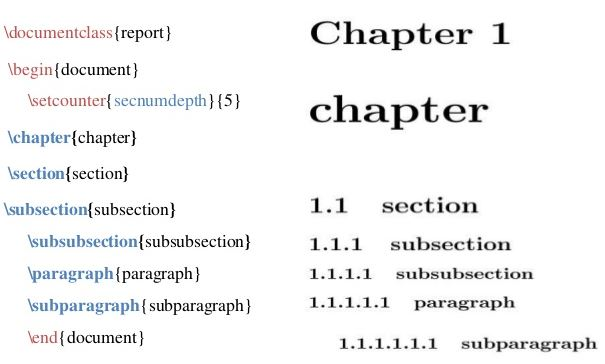
\includegraphics[width=0.50\textwidth]{gambar/dokumen}}
	\caption{dokumen}
	\label{dokumen}
\end{figure}

\vspace{50pt}
\hspace{0.50in} Sedangkan dokumen kelas report dan book selain memiliki perintah-perintah di atas memiliki juga perintah :
 \par
{\fontsize{10pt}{10pt}\selectfont  $  \setminus  $part $  \{  $... $  \}  $}
 \par
\vspace{9pt}

{\fontsize{10pt}{10pt}\selectfont  $  \setminus  $chapter $  \{  $... $  \}  $}
 \par
\vspace{9pt}
{\fontsize{10pt}{10pt}\selectfont  $  \setminus  $frontmatter}
 \par
\vspace{9pt}
{\fontsize{10pt}{10pt}\selectfont  $  \setminus  $mainmatter}
 \par
\vspace{9pt}
{\fontsize{10pt}{10pt}\selectfont  $  \setminus  $backmatter}
 \par
\vspace{12pt}
\hspace{0.50in} Argumen yang diberikan pada perintah-perintah ini adalah nama bab, subbab, dll. Dalam naskah buku yang dituliskan dengan kelas dokumen book, fronmatter digunakan untuk menandai halaman judul, daftar isi, kata pengantar, daftar gambar, dsb. Sedangkan mainmatter digunakan untuk menandai bagian tulisan utama, dan backmatter untuk menandai daftar pustaka, indeks, daftar istilah, dsb. Perintah  $  \setminus  $chapter,  $  \setminus  $section,  $  \setminus  $subsection, dan  $  \setminus  $subsubsection secara otomatis memberikan nomor pada nama bagian, bab, dsb. Jika nomor ini tidak diinginkan, maka perintah yang ekivalen adalah  $  \setminus  $chapter*,  $  \setminus  $section*,  $  \setminus  $subsection*, dan  $  \setminus  $subsubsection*.
 \par
\vspace{12pt}
\hspace{0.50in} Perintah bagian diberi nomor dan akan muncul dalam daftar isi dokumen. Paragraf tidak diberi nomor dan tidak akan ditampilkan dalam daftar isi. Berikut contoh output menggunakan bagian:
 \par
1 Section
 \par
~~ Hello World!
 \par
~~~~~ 1.1 Subsection
 \par
~~~~~~~~~~~~ Structuring a document is easy
 \par
\vspace{12pt}
\hspace{0.50in} Untuk mendapatkan hasil ini, Anda hanya perlu menambahkan beberapa baris ke program kami dari pelajaran 1:
 \par
 $  \setminus  $documentclass $  \{  $article $  \}  $
 \par
\vspace{12pt}
 $  \setminus  $title $  \{  $Title of my document $  \}  $
 \par
 $  \setminus  $date $  \{  $2013-09-01 $  \}  $
 \par
 $  \setminus  $author $  \{  $John Doe $  \}  $
 \par
\vspace{12pt}
 $  \setminus  $begin $  \{  $document $  \}  $
 \par
\vspace{12pt}
 $  \setminus  $maketitle
 \par
 $  \setminus  $pagenumbering $  \{  $gobble $  \}  $
 \par

 $  \setminus  $newpage
 \par
 $  \setminus  $pagenumbering $  \{  $arabic $  \}  $
 \par
\vspace{12pt}
 $  \setminus  $section $  \{  $Section $  \}  $
 \par
\vspace{12pt}
Hello World!
 \par
\vspace{12pt}
 $  \setminus  $subsection $  \{  $Subsection $  \}  $
 \par
\vspace{12pt}
Structuring a document is easy!
 \par
\vspace{12pt}
 $  \setminus  $end $  \{  $document $  \}  $
 \par
\vspace{14pt}
Gambar berikut menunjukkan struktur hirarkis dari semua elemen:
 \par
1. Section
 \par
~~~ Hello World
 \par
~~~~ 1.1 Subsection
 \par
~~~~~~~~~~ Structuring a document is easy!
 \par
~~~~~~~~~ 1.1 Subsection
 \par
~~~~~~~~~~~~~~~ More Text
 \par
~~~~~~~~~~~~~~~ Paragraph ~~~~~~~~~~~~ Some more text
 \par
~~~~~~~~~~~~~~~ Subparagraph ~~~~~~~ Even more text \par
2. Another Section
 \par
\hspace{0.50in} Saya telah menggunakan kode berikut untuk mendapatkan output ini:
 \par
 $  \setminus  $documentclass $  \{  $article $  \}  $
 \par
\vspace{12pt}
 $  \setminus  $begin $  \{  $document $  \}  $
 \par
\vspace{12pt}
 $  \setminus  $section $  \{  $Section $  \}  $
 \par
\vspace{12pt}
Hello World!
 \par
\vspace{12pt}
 $  \setminus  $subsection $  \{  $Subsection $  \}  $
 \par
\vspace{12pt}
Structuring a document is easy!
 \par
\vspace{12pt}
 $  \setminus  $subsubsection $  \{  $Subsubsection $  \}  $
 \par
\vspace{12pt}
More text.
 \par
\vspace{12pt}
 $  \setminus  $paragraph $  \{  $Paragraph $  \}  $
 \par
\vspace{12pt}
Some more text.
 \par
\vspace{12pt}
 $  \setminus  $subparagraph $  \{  $Subparagraph $  \}  $
 \par
\vspace{12pt}
Even more text.
 \par
\vspace{12pt}
 $  \setminus  $section $  \{  $Another section $  \}  $
 \par
\vspace{12pt}
 $  \setminus  $end $  \{  $document $  \}  $
 \par
\vspace{12pt}
\vspace{12pt}
Contoh struktur dokumen berkelas article dan book :
 \par
{\fontsize{10pt}{10pt}\selectfont  $  \setminus  $documentclass $  \{  $article $  \}  $}
 \par
\vspace{10pt}
{\fontsize{10pt}{10pt}\selectfont  $  \setminus  $usepackage $  \{  $... $  \}  $}
 \par
\vspace{10pt}
{\fontsize{10pt}{10pt}\selectfont  $  \setminus  $begin $  \{  $document $  \}  $}
 \par
\vspace{10pt}
{\fontsize{10pt}{10pt}\selectfont  $  \setminus  $maketitle}
 \par
\vspace{10pt}
{\fontsize{10pt}{10pt}\selectfont  $  \setminus  $section $  \{  $... $  \}  $}
 \par
\vspace{10pt}
{\fontsize{10pt}{10pt}\selectfont  $  \setminus  $section $  \{  $... $  \}  $}
 \par
\vspace{10pt}
{\fontsize{10pt}{10pt}\selectfont  $  \setminus  $subsection $  \{  $... $  \}  $}
 \par
\vspace{10pt}
{\fontsize{10pt}{10pt}\selectfont  $  \setminus  $subsubsection $  \{  $... $  \}  $}
 \par
\vspace{10pt}
{\fontsize{10pt}{10pt}\selectfont  $  \setminus  $section}
 \par
\vspace{10pt}
{\fontsize{10pt}{10pt}\selectfont  $  \setminus  $end $  \{  $document $  \}  $}
 \par
\vspace{12pt}
\hspace{0.50in} LaTeX dapat menyusun dokumen menjadi beberapa bagian dengan sangat mudah. Hal ini karena LaTeX memiliki format yang konsisten di seluruh kertas. Berikut perintah-perintah latex, seperti:
 \begin{itemize}
\item part \par
\textit{part} berfungsi untuk membuat pembagian bab, biasanya dibuat dalam halaman yang terpisah. Adapun penggunaannya adalah sebagai berikut:

{\fontsize{10pt}{10pt}\selectfont ~~  $  \setminus  $part $  \{  $[Judul] $  \}  $}
 \par
\item chapter \par
\textit{chapter} merupakan bab utama yang memuat judul. Penggunaannya demikian:
\par
{\fontsize{10pt}{10pt}\selectfont ~~  $  \setminus  $chapter $  \{  $[Judul] $  \}  $}
\par
\item section \par
\textit{section} merupakan pasal dari suatu bab. Contoh penggunaannya adalah sebagai berikut:\
 \par
{\fontsize{10pt}{10pt}\selectfont ~~~  $  \setminus  $section $  \{  $[Judul] $  \}  $}
 \par
\item subsection \par
subsection \textit{subsection} berfungsi untuk membuat sub pasal atau pasal baru di bawah judul pasal.
 \par
{\fontsize{10pt}{10pt}\selectfont ~~  $  \setminus  $subsection $  \{  $Judul $  \}  $}
 \par
\textit{subsubsection} berfungsi untuk membuat sub pasal di bawahnya lagi dari sub pasal yang ada.
 \par
{\fontsize{10pt}{10pt}\selectfont ~~  $  \setminus  $subsubsection* $  \{  $Judul $  \}  $}
 \par
 \item paragraph \par
\textit{paragraph} berguna untuk membuat alinea kalimat, cara penggunaannya adalah sebagai berikut:
 \par
{\fontsize{10pt}{10pt}\selectfont ~~  $  \setminus  $paragraph $  \{  $kalimat $  \}  $}
 \par
\item subparagraph \par
\textit{subpragraph} berfungsi untuk membuat alinea baru di dalam alinea yang sudah ada. Cara penggunaannya adalah demikian:
 \par
{\fontsize{10pt}{10pt}\selectfont ~~  $  \setminus  $subparagraph $  \{  $kalimat $  \}  $}
 \par
 \vspace{12pt}
Contoh struktur dokumen berikut ini:
 \par
{\fontsize{10pt}{10pt}\selectfont  $  \setminus  $part $  \{  $Memulai LATEX $  \}  $  $  \%  $ ini adalah contoh penggunaan part}
 \par
{\fontsize{10pt}{10pt}\selectfont ~~~~~  $  \setminus  $chapter $  \{  $Menggunakan LATEX $  \}  $  $  \%  $ ini adalah contoh penggunaan chapter}
 \par
{\fontsize{10pt}{10pt}\selectfont ~~~~~~~~~~~  $  \setminus  $section $  \{  $Penggunaan Class dalam penulisan dokumen $  \}  $}
 \par
{\fontsize{10pt}{10pt}\selectfont  \hspace*{0.64in} ~  \hspace*{0.64in}  \hspace*{0.64in}  $  \%  $ ini adalah contoh penggunaan section}
 \par
{\fontsize{10pt}{10pt}\selectfont ~~~~~~~~~~~~~~~~ $  \setminus  $subsection $  \{  $Penyertaan Package $  \}  $  }
 \par
{\fontsize{10pt}{10pt}\selectfont  \hspace*{0.64in}  \hspace*{0.64in}  \hspace*{0.64in}  $  \%  $ ini adalah contoh penggunaan subsection}
 \par
{\fontsize{10pt}{10pt}\selectfont  \hspace*{0.64in}  \hspace*{0.64in}  \hspace*{0.64in}  $  \setminus  $paragraph $  \{  $Penyertaan package berguna untuk menambahkan fungsi }
 \par
{\fontsize{10pt}{10pt}\selectfont  \hspace*{0.64in}  \hspace*{0.64in}  \hspace*{0.64in} kedalam dokumen/naskah yang kita buat. Bentuk penulisannya }
 \par
{\fontsize{10pt}{10pt}\selectfont  \hspace*{0.64in}  \hspace*{0.64in}  \hspace*{0.64in} adalah sebagai berikut: $  \}  $}
 \par
{\fontsize{10pt}{10pt}\selectfont   \hspace*{0.64in}  \hspace*{0.64in}  \hspace*{0.64in}  \hspace*{0.64in}  $  \%  $ ini adalah contoh penggunaan paragraph}
 \par
\end{itemize}
\vspace{10pt}
\subsection{Komentar}
 \par
\hspace{0.50in} Fungsi dari komentar adalah untuk menampilkan catatan dari naskah yang telah Anda buat, namun tidak ditampilkan pada saat file dicetak. Contoh penggunaan nya adalah sebagai berikut:
 \par
{\fontsize{10pt}{10pt}\selectfont  $  \setminus  $documentclass[12pt,a4paper,oneside,bahasa,dvips] $  \{  $book $  \}  $}
 \par
{\fontsize{10pt}{10pt}\selectfont  $  \setminus  $begin $  \{  $document $  \}  $}
 \par
{\fontsize{10pt}{10pt}\selectfont Halo, ini adalah contoh penulisan menggunakan LaTeX.}
 \par
{\fontsize{10pt}{10pt}\selectfont ukuran font dari naskah ini adalah 12. Pencetakan akan menggunakan}
 \par
{\fontsize{10pt}{10pt}\selectfont kertas A4, yang akan dicetak dalam satu sisi. Naskah ini berbentuk bu}
 \par
{\fontsize{10pt}{10pt}\selectfont dan akan ditampilkan kedalam bahasa Indonesia.}
 \par
{\fontsize{10pt}{10pt}\selectfont komentar ini tidak akan ditampilkan pada saat dilakukan pencetakan}
 \par
{\fontsize{10pt}{10pt}\selectfont naskah.}
 \par
{\fontsize{10pt}{10pt}\selectfont  $  \setminus  $end $  \{  $document $  \}  $}
 \par
\subsection{Membuat Judul Dokumen}
 \par
Untuk judul dokumen, perintahnya adalah sebagai berikut:
 \par
{\fontsize{10pt}{10pt}\selectfont  $  \setminus  $title $  \{  $ $  \}  $}
 \par
{\fontsize{10pt}{10pt}\selectfont  $  \setminus  $maketitle}
 \par
\vspace{12pt}
Adapun contohnya adalah sebagai berikut:
 \par
{\fontsize{10pt}{10pt}\selectfont  $  \setminus  $documentclass[12pt,a4paper,oneside,bahasa,dvips] $  \{  $book $  \}  $}
 \par
{\fontsize{10pt}{10pt}\selectfont  $  \setminus  $title $  \{  $Membuat Dokumen dengan  $  \setminus  $LaTeX $  \{  $ $  \}  $ $  \}  $}
 \par
{\fontsize{10pt}{10pt}\selectfont  $  \setminus  $begin $  \{  $document $  \}  $}
 \par
{\fontsize{10pt}{10pt}\selectfont  $  \setminus  $maketitle}
 \par
\vspace{10pt}
{\fontsize{10pt}{10pt}\selectfont Halo, ini adalah contoh penulisan menggunakan LaTeX, dengan ukuran font Pencetakan akan menggunakan kertas A4, yang akan dicetak dalam satu sis Naskah ini berbentuk buku dan akan ditampilkan kedalam bahasa Indonesia judul akan ditampilkan secara otomatis pada awal dokumen ketika dokumen dikonversi ke format DVI,HTML, ataupun PDF.  $  \setminus  $end $  \{  $document $  \}  $} 

\subsection{Memisahkan Baris} \par
Untuk memisahkan baris, Anda bisa menggunakan perintah sebagai berikut: \par
 $  \setminus  $ $  \setminus  $ \par
atau \par
{\fontsize{10pt}{10pt}\selectfont  $  \setminus  $newline} \par
\vspace{12pt}
Adapun contoh penggunaannya adalah demikian: \par
Contoh 1: \par
{\fontsize{10pt}{10pt}\selectfont  $  \setminus  $documentclass[12pt,a4paper,oneside,bahasa,dvips] $  \{  $book $  \}  $} \par
{\fontsize{10pt}{10pt}\selectfont  $  \setminus  $begin $  \{  $document $  \}  $} \par
\vspace{10pt}
{\fontsize{10pt}{10pt}\selectfont Halo, ini adalah contoh penulisan menggunakan LaTeX, dengan ukuran font Pencetakan akan menggunakan kertas A4, yang akan dicetak dalam satu sis Naskah ini berbentuk buku dan akan ditampilkan kedalam bahasa Indonesia} \par
\vspace{10pt}
{\fontsize{10pt}{10pt}\selectfont Tulisan ini akan ditampilkan dengan penambahan satu baris.} \par
{\fontsize{10pt}{10pt}\selectfont  $  \setminus  $end $  \{  $document $  \}  $} \par
\vspace{10pt}
Contoh 2: \par
{\fontsize{10pt}{10pt}\selectfont  $  \setminus  $documentclass[12pt,a4paper,oneside,bahasa,dvips] $  \{  $book $  \}  $} \par
{\fontsize{10pt}{10pt}\selectfont  $  \setminus  $begin $  \{  $document $  \}  $} \par
\vspace{10pt}
{\fontsize{10pt}{10pt}\selectfont Halo, ini adalah contoh penulisan menggunakan LaTeX, dengan ukuran font Pencetakan akan menggunakan kertas A4, yang akan dicetak dalam satu sis Naskah ini berbentuk buku dan akan ditampilkan kedalam bahasa Indonesia} \par
\vspace{10pt}
{\fontsize{10pt}{10pt}\selectfont  $  \setminus  $linebreak} \par
{\fontsize{10pt}{10pt}\selectfont Tulisan ini akan ditampilkan dengan penambahan satu baris.} \par

{\fontsize{10pt}{10pt}\selectfont  $  \setminus  $end $  \{  $document $  \}  $}
 \par

\subsection{Berpindah Halaman}
 \par
Untuk berpindah halaman, Anda bisa menggunakan perintah sebagai berikut: \par
\begin{equation}
newpage
\end{equation}

\vspace{9pt}
Contohnya adalah sebagai berikut \par
{\fontsize{10pt}{10pt}\selectfont  $  \setminus  $documentclass[12pt,a4paper,oneside,bahasa,dvips] $  \{  $book $  \}  $} \par
{\fontsize{10pt}{10pt}\selectfont  $  \setminus  $title $  \{  $Membuat Dokumen dengan  $  \setminus  $LaTeX $  \{  $ $  \}  $ $  \}  $} \par
{\fontsize{10pt}{10pt}\selectfont  $  \setminus  $author $  \{  $R. Kresno Aji (masaji@ai.co.id) $  \}  $} \par
{\fontsize{10pt}{10pt}\selectfont  $  \setminus  $date $  \{  $17 Agustus 2004 $  \}  $} \par
{\fontsize{10pt}{10pt}\selectfont  $  \setminus  $begin $  \{  $document $  \}  $} \par
{\fontsize{10pt}{10pt}\selectfont  $  \setminus  $maketitle} \par
\vspace{10pt}
{\fontsize{10pt}{10pt}\selectfont Halo, ini adalah contoh penulisan menggunakan LaTeX, dengan ukuran font Pencetakan akan menggunakan kertas A4, yang akan dicetak dalam satu sis Naskah ini berbentuk buku dan akan ditampilkan kedalam bahasa Indonesia judul akan ditampilkan secara otomatis pada awal dokumen ketika dokumen dikonversi ke format DVI,HTML, ataupun PDF.} \par
\vspace{10pt}
{\fontsize{10pt}{10pt}\selectfont  $  \setminus  $newpage} \par
{\fontsize{10pt}{10pt}\selectfont  $  \setminus  $chapter $  \{  $Halaman Baru $  \}  $} \par
{\fontsize{10pt}{10pt}\selectfont  $  \setminus  $end $  \{  $document $  \}  $} \par

\subsection{Environtment} \par
LATEX menyediakan environmen yang berupa: \par
* Itemize \par
~~ berfungsi untuk membuat daftar yang tidak memiliki urutan. \par
* Enumerate \par
~~ berfungsi untuk membuat daftar yang berurutan. \par
* Flushleft \par
~~ untuk membuat kalimat rata kiri. \par
* Center \par
~~ berfungsi untuk membuat kalimat dengan format center. \par
* Flushright \par
~~ berfungsi untuk membuat kalimat rata kanan. \par
* Footnote \par
~~ berfungsi untuk membuat catatan kaki. \par
* Verbatim \par
~~ berfungsi untuk membuat kalimat / karakter yang ditulis \par
* Table
 \par
~~ berfungsi untuk membuat tabel.  \par 
\begin{enumerate}
\item  Pembuatan daftar berurutan \par
Untuk membuat daftar yang berurutan, Anda bisa menggunakan perintah berikut ini: \par
{\fontsize{10pt}{10pt}\selectfont  $  \setminus  $begin $  \{  $enumerate $  \}  $} \par
{\fontsize{10pt}{10pt}\selectfont  $  \setminus  $item} \par
{\fontsize{10pt}{10pt}\selectfont  $  \setminus  $end $  \{  $enumerate $  \}  $} \par
\vspace{12pt}
Contohnya adalah demikian: \par
{\fontsize{10pt}{10pt}\selectfont  $  \setminus  $documentclass[12pt,a4paper,oneside,bahasa,dvips] $  \{  $book $  \}  $} \par
{\fontsize{10pt}{10pt}\selectfont  $  \setminus  $begin $  \{  $document $  \}  $} \par
\vspace{10pt}
{\fontsize{10pt}{10pt}\selectfont Halo, ini adalah contoh penulisan menggunakan LaTeX, dengan ukuran font Pencetakan akan menggunakan kertas A4, yang akan dicetak dalam satu sis Naskah ini berbentuk buku dan akan ditampilkan kedalam bahasa Indonesia Daftar secara berurutan akan ditampilkan secara otomatis pada awal {\fontsize{9pt}{9pt}\selectfont dokumen ketika dokumen dikonversi ke format DVI,HTML, ataupun PDF.}} \par
\vspace{12pt}
{\fontsize{10pt}{10pt}\selectfont Pada bab ini, kita akan membahas:} \par
{\fontsize{10pt}{10pt}\selectfont  $  \setminus  $begin $  \{  $enumerate $  \}  $} \par
{\fontsize{10pt}{10pt}\selectfont  $  \setminus  $item item satu} \par
{\fontsize{10pt}{10pt}\selectfont  $  \setminus  $item item dua} \par
{\fontsize{10pt}{10pt}\selectfont  $  \setminus  $end $  \{  $enumerate $  \}  $} \par
{\fontsize{10pt}{10pt}\selectfont  $  \setminus  $end $  \{  $document $  \}  $} \par
\vspace{10pt}
\noindent 
\item Penggunaan rata kiri, rata kanan dan center \par
\noindent 
~~~~ Untuk membuat dokumen LATEX menjadi rata kiri perintahnya adalah demikian: \par
{\fontsize{10pt}{10pt}\selectfont  $  \setminus  $begin $  \{  $flushleft $  \}  $} \par
{\fontsize{10pt}{10pt}\selectfont [kalimat]} \par
{\fontsize{10pt}{10pt}\selectfont  $  \setminus  $end $  \{  $flushleft $  \}  $} \par
\vspace{12pt}
Contohnya adalah sebagai berikut: \par
{\fontsize{10pt}{10pt}\selectfont  $  \setminus  $documentclass[12pt,a4paper,oneside,bahasa,dvips] $  \{  $book $  \}  $} \par
{\fontsize{10pt}{10pt}\selectfont  $  \setminus  $begin $  \{  $document $  \}  $} \par
{\fontsize{10pt}{10pt}\selectfont  $  \setminus  $begin $  \{  $flushleft $  \}  $} \par
\vspace{9pt}
{\fontsize{10pt}{10pt}\selectfont Halo, ini adalah contoh penulisan menggunakan LaTeX, dengan ukuran font Pencetakan akan menggunakan kertas A4, yang akan dicetak dalam satu sis Naskah ini berbentuk buku dan akan ditampilkan kedalam bahasa Indonesia dan berada di sebelah kiri.} \par
\vspace{9pt}
{\fontsize{10pt}{10pt}\selectfont  $  \setminus  $end $  \{  $flushleft $  \}  $} \par
{\fontsize{10pt}{10pt}\selectfont  $  \setminus  $end $  \{  $document $  \}  $} \par
\vspace{12pt}
Untuk membuat dokumen LATEX menjadi rata kanan, perintahnya adalah demikian: \par
{\fontsize{10pt}{10pt}\selectfont  $  \setminus  $begin $  \{  $flushright $  \}  $} \par
{\fontsize{10pt}{10pt}\selectfont [kalimat]} \par
{\fontsize{10pt}{10pt}\selectfont  $  \setminus  $end $  \{  $flushright $  \}  $} \par
\vspace{12pt}
Contohnya adalah sebagai berikut: \par
{\fontsize{10pt}{10pt}\selectfont  $  \setminus  $documentclass[12pt,a4paper,oneside,bahasa,dvips] $  \{  $book $  \}  $} \par
{\fontsize{10pt}{10pt}\selectfont  $  \setminus  $begin $  \{  $document $  \}  $} \par
{\fontsize{10pt}{10pt}\selectfont  $  \setminus  $begin $  \{  $flushright $  \}  $} \par
\vspace{10pt}
{\fontsize{10pt}{10pt}\selectfont Halo, ini adalah contoh penulisan menggunakan LaTeX, dengan ukuran font Pencetakan akan menggunakan kertas A4, yang akan dicetak dalam satu sis Naskah ini berbentuk buku dan akan ditampilkan kedalam bahasa Indonesia dan terletak rata kanan.} \par
\vspace{10pt}
{\fontsize{10pt}{10pt}\selectfont  $  \setminus  $end $  \{  $flushright $  \}  $} \par
{\fontsize{10pt}{10pt}\selectfont  $  \setminus  $end $  \{  $document $  \}  $} \par
\vspace{10pt}
Untuk membuat dokumen LATEX menjadi center perintahnya adalah demikian: \par
{\fontsize{10pt}{10pt}\selectfont  $  \setminus  $begin $  \{  $center $  \}  $} \par
{\fontsize{10pt}{10pt}\selectfont [kalimat]} \par
{\fontsize{10pt}{10pt}\selectfont  $  \setminus  $end $  \{  $center $  \}  $} \par
\vspace{10pt}
Contohnya adalah sebagai berikut: \par
{\fontsize{10pt}{10pt}\selectfont  $  \setminus  $documentclass[12pt,a4paper,oneside,bahasa,dvips] $  \{  $book $  \}  $ \hspace*{0.5in} } \par
{\fontsize{10pt}{10pt}\selectfont  $  \setminus  $begin $  \{  $document $  \}  $} \par
{\fontsize{10pt}{10pt}\selectfont  $  \setminus  $begin $  \{  $center $  \}  $} \par
\vspace{9pt}
{\fontsize{10pt}{10pt}\selectfont Halo, ini adalah contoh penulisan menggunakan LaTeX, dengan ukuran font Pencetakan akan menggunakan kertas A4, yang akan dicetak dalam satu sis Naskah ini berbentuk buku dan akan ditampilkan kedalam bahasa Indonesia dan terletak center.} \par
\vspace{9pt}
{\fontsize{10pt}{10pt}\selectfont  $  \setminus  $end $  \{  $center $  \}  $} \par
{\fontsize{10pt}{10pt}\selectfont  $  \setminus  $end $  \{  $document $  \}  $} \par
\vspace{14pt}
\noindent 
\item Pembuatan footnote \par
Untuk pembuatan footnote pada dokumen LATEX, Anda bisa memberikan perintah sebagai berikut:  \par
\vspace{12pt}
{\fontsize{10pt}{10pt}\selectfont  $  \setminus  $footnote $  \{  $ ...  $  \}  $} \par
\vspace{12pt}
Contohnya adalah demikian: \par
{\fontsize{10pt}{10pt}\selectfont  $  \setminus  $documentclass[12pt,a4paper,oneside,bahasa,dvips] $  \{  $book $  \}  $} \par
{\fontsize{10pt}{10pt}\selectfont  $  \setminus  $begin $  \{  $document $  \}  $} \par
\vspace{12pt}
{\fontsize{10pt}{10pt}\selectfont Halo, ini adalah contoh penulisan menggunakan LaTeX, dengan ukuran font Pencetakan akan menggunakan kertas A4, yang akan dicetak dalam satu sis Naskah ini berbentuk buku dan akan ditampilkan kedalam bahasa Indonesia  $  \setminus  $footnote $  \{  $Ini adalah contoh penggunaan footnote $  \}  $} \par
\vspace{9pt}
{\fontsize{10pt}{10pt}\selectfont  $  \setminus  $end $  \{  $document $  \}  $} \par
\vspace{10pt}
\noindent 
\item  Penulisan apa adanya dengan verbatim \par
Seperti halnya pada penulisan dalam format HTML, dengan menggunakan tag < pre >. LATEX juga menyediakan fasilitas ini. Adapun formatnya adalah sebagai berikut: \par
begin $  \{  $verbatim $  \}  $ \par
[kalimat] \par
end $  \{  $verbatim $  \}  $ \par
\vspace{8pt}
\vspace{8pt}
Contohnya adalah sebagai berikut: \par
{\fontsize{10pt}{10pt}\selectfont  $  \setminus  $begin $  \{  $verbatim $  \}  $} \par
{\fontsize{10pt}{10pt}\selectfont  $  \setminus  $documentclass[12pt,a4paper,oneside,bahasa,dvips] $  \{  $book $  \}  $} \par
{\fontsize{10pt}{10pt}\selectfont  $  \setminus  $begin $  \{  $document $  \}  $} \par
\vspace{10pt}
{\fontsize{10pt}{10pt}\selectfont Pada bab ini, kita akan membahas:} \par
{\fontsize{10pt}{10pt}\selectfont  $  \setminus  $begin $  \{  $itemize $  \}  $} \par
{\fontsize{10pt}{10pt}\selectfont  $  \setminus  $item item satu} \par
{\fontsize{10pt}{10pt}\selectfont  $  \setminus  $item item dua} \par
{\fontsize{10pt}{10pt}\selectfont  $  \setminus  $end $  \{  $itemize $  \}  $} \par
{\fontsize{10pt}{10pt}\selectfont  $  \setminus  $end $  \{  $document $  \}  $} \par
{\fontsize{10pt}{10pt}\selectfont end $  \{  $verbatim $  \}  $} \par
\vspace{10pt}
{\fontsize{10pt}{10pt}\selectfont Maka jika dilakukan pencetakan, hasilnya akan tampak sebagai berikut:} \par
{\fontsize{10pt}{10pt}\selectfont Pada bab ini, kita akan membahas:} \par
{\fontsize{10pt}{10pt}\selectfont  $  \setminus  $begin $  \{  $itemize $  \}  $} \par
{\fontsize{10pt}{10pt}\selectfont  $  \setminus  $item item satu} \par
{\fontsize{10pt}{10pt}\selectfont  $  \setminus  $item item dua} \par
{\fontsize{10pt}{10pt}\selectfont  $  \setminus  $end $  \{  $itemize $  \}  $} \par
\vspace{10pt}
\noindent 
\item Pembuatan Tabel \par
 Untuk membuat tabel pada dokumen LATEX, perintahnya adalah sebagai berikut: \par
{\fontsize{10pt}{10pt}\selectfont  $  \setminus  $begin $  \{  $tabular $  \}  $} \par
{\fontsize{10pt}{10pt}\selectfont  $  \setminus  $end $  \{  $tabular $  \}  $} \par
\vspace{12pt}
Untuk jelasnya, Anda bisa meniru langkah di bawah ini: \par
{\fontsize{10pt}{10pt}\selectfont  $  \setminus  $hline} \par
{\fontsize{10pt}{10pt}\selectfont  $  \setminus  $begin $  \{  $tabular $  \}  $ $  \{  $ $  \vert  $c $  \vert  $c $  \vert  $c $  \vert  $ $  \}  $} \par
{\fontsize{10pt}{10pt}\selectfont No.  $  \&  $  $  \setminus  $bf Uraian  $  \&  $ Jumlah  $  \setminus  $ $  \setminus  $} \par
{\fontsize{10pt}{10pt}\selectfont  $  \setminus  $hline} \par
\begin{itemize}
\item {\fontsize{10pt}{10pt}\selectfont  $  \&  $ Pembelian alat-alat kantor  $  \&  $ Rp. 250.000  $  \setminus  $ $  \setminus  $  $  \setminus  $cline $  \{  $2-2 $  \}  $}\end{itemize}
 \par
{\fontsize{10pt}{10pt}\selectfont  $  \setminus  $hline} \par
{\fontsize{10pt}{10pt}\selectfont  $  \setminus  $end $  \{  $tabular $  \}  $} \par
\vspace{12pt}
\noindent 
\item Mengubah bentuk dan ukuran font \par
Ada beberapa mode perubahan font pada LATEX, seperti bisa Anda lihat pada penjelasan berikut ini:
 \par
\vspace{12pt}
Untuk memperkecil huruf, perintahnya adalah demikian: \par
 $  \setminus  $small \par
\vspace{12pt}
Untuk memperbesar huruf, perintah sebagai berikut: \par
{\fontsize{10pt}{10pt}\selectfont  $  \setminus  $large} \par
{\fontsize{10pt}{10pt}\selectfont  $  \setminus  $LARGE} \par
{\fontsize{10pt}{10pt}\selectfont  $  \setminus  $Huge} \par
\vspace{12pt}
Contohnya adalah demikian: \par
\begin{verbatim}
\documentclass[12pt] {article} 
\begin {document} 
\end {document}
\end{verbatim}
\vspace{8pt}
\item Membuat daftar pustaka \par
Akhir dari pembuatan dokumen atau naskah ilmiah adalah dengan membuat daftar pustaka atau referensi. Pada LaTeX, hal ini sudah tersedia. Anda hanya perlu menggunakannya saja. Adapun perintahnya adalah sebagai berikut: \par
{\fontsize{10pt}{10pt}\selectfont  $  \setminus  $bibliographystyle $  \{  $plain $  \}  $} \par
{\fontsize{10pt}{10pt}\selectfont  $  \setminus  $begin $  \{  $thebibliography $  \}  $ $  \{  $Refference $  \}  $} \par
{\fontsize{10pt}{10pt}\selectfont  $  \setminus  $bibitem} \par
{\fontsize{10pt}{10pt}\selectfont  $  \setminus  $end $  \{  $thebibliography $  \}  $} \par
\vspace{12pt}
Untuk jelasnya, Anda bisa melihat contoh di bawah ini: \par
\begin{verbatim}
\bibliographystyle {plain}
\begin {thebibliography} {Refference}
\bibitem A Guide to LaTex}
\end {thebibliography} 
\end{verbatim}
\end{enumerate}
